%------------------------------------------------------------------------------
%	CAPITOLO 13
%------------------------------------------------------------------------------

\chapter{I paletti bianchi delle strade}
\subsection{I paletti bianchi delle strade}
Per chi non lo sapesse sembrerebbe un'invenzione dell'Azienda Stradale, dovuta allo sviluppo automobilistico, ma così non è. Sotto al governo papale verso il 1850, nella magistratura comunale di Alfonsine si discuteva e si doveva approvare la prima illuminazione pubblica.\\
\indent Il membro \index[Personaggi]{Bagnara Giovanni}Bagnara\footnote{\textbf{Giovanni Bagnara}, fu più volte membro della giunta comunale. Fu il padre di Cassiano\index[Personaggi]{Bagnara Cassiano}, il quale fu vittima di un atto di brigantaggio  da parte della `Ligaza di Trentesì' la sera del 20 novembre 1862 e fu ucciso. Erano i proprietari della casa di Vincenzo Monti} fece la proposta di imbiancare le teste dei pali stradali, perché ciascuno rincasando alla sera avesse un punto di mira per seguire la buona strada.\\
\indent Per molto tempo tutti risero della trovata, ma ora perché è morto da 70 anni... il mondo deve dargli ragione.

\subsection{Le ragazze non devono saper scrivere}
Il \index[Personaggi]{Bagnara Giovanni}Bagnara aveva profondamente radicate le sue convinzioni morali e politiche. Secondo lui le donne non dovevano imparare a leggere e scrivere... perché non scrivessero al fidanzato! La maniera di repressione era, si vede, molto radicale.\\

\subsection{Una vacca morta}
Sempre parlando del nostro uomo che in fondo era buonissimo, diremo ancora.\\
\indent Un giorno un suo contadino gli porta la brutta nuova che gli è morta una vacca. In altre occasioni si sarebbe vivamente accorato\footnote{Dispiaciuto}, per l'affezione che aveva alle bestie e per il danno. Nel caso, non si scompose e rispose:\\
\indent <<L'è l'istes ui aveva la su mitè nec Mingàz\footnote{<<È lo stesso, vi aveva la sua metà anche Mingazzi>>}>>. \\
\indent Si vede che per lui il danno comune era una gioia! E pensare che col Mingazzi\footnote{Probabilmente si parla di \index[Personaggi]{Mingazzi Fedele}Fedele Mingazzi, il nonno paterno di Stefano oppure il padre, Natale Mingazzi} erano amiconi.


 \begin{figure}[htb]
    \centering
    %\vspace{-0.7cm}
    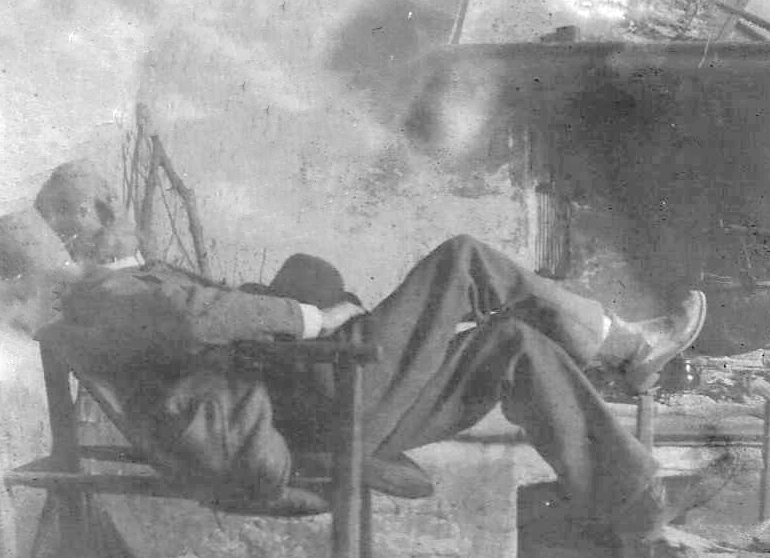
\includegraphics[width=\textwidth]{natalemingazzi}
    \caption[Natale Mingazzi in casa]{\textbf{Natale Mingazzi}\index[Personaggi]{Mingazzi Natale}, il padre di Stefano. Aveva un allevamento di bachi da seta, come ho scoperto leggendo le lettere che la sua futura moglie Mariannina gli inviava da Bologna. In una di quelle lettere si diceva dispiaciuta per il fidanzato sapendo che le larve erano uscite dalla finestra. \label{fig:natalemingazzi}}
    %\vspace{-0.3cm}
\end{figure}